\documentclass{beamer}
%\usetheme{Luebeck}
\usepackage{graphicx}
\usepackage{xcolor}
\usepackage{ifsym}
\usepackage{latexsym}
\usepackage{graphicx}
\usepackage{amsmath}
\usepackage{amssymb}
\usepackage{tipa}
\usepackage{textcomp}
\usepackage{tikz}
\usepackage{pgf}
\usepackage{pgfplots}
\usepackage{subfig}
\usepackage{changepage}
\pgfplotsset{width=9cm,compat=1.8}
\usetikzlibrary{arrows,automata}
%\usefonttheme{serif}
\usepackage{bbding}

%\usepackage{flexbib}
\usepackage{gb4e}
%combinación de themes para los frames. 
\usecolortheme{nautico}
\usecolortheme{whale}
\usecolortheme{orchid}



\definecolor{wine}{rgb}{0.55,0,0}
\definecolor{forestgreen}{rgb}{0.13,0.55,0.13}


\begin{document}

\resetcounteronoverlays{exx}  %%to prevent the package gb4e to increase sample numbers while using \pause in lists. 

\title{\color{white}\textrm{\emph{Fleiss' Kappa Results}}}
\author{\small{Seth-David Donald Dworman \\sdworman@brandeis.edu}}
\institute{\color{black}\textrm{Brandeis Lab for Linguistics and Computation}}
\date{\small{November 25th, 2014}}
\maketitle

\begin{frame}{Tokens}
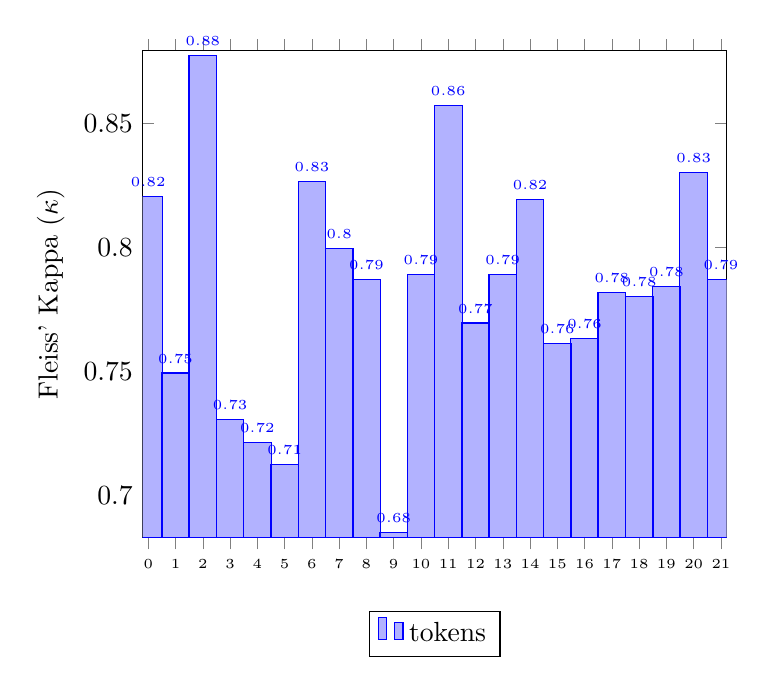
\begin{tikzpicture}
\begin{axis}[
    ybar,
    enlargelimits=0.01,
    legend style={at={(0.5,-0.15)},
      anchor=north,legend columns=-1},
    ylabel={Fleiss' Kappa ($\kappa$)},
    symbolic x coords={0,1,2,3,4,5,6,7,8,9,10,11,12,13,14,15,16,17,18,19,20,21},
    xtick=data, xticklabel style={font=\tiny},
    nodes near coords,
    every node near coord/.append style={font=\tiny},
    nodes near coords align={vertical},
    ]
\addplot coordinates {(0,0.820634615371) (1,0.749387104566) (2,0.877447627014) (3,0.730605521817) (4,0.721264576953) (5,0.712448104015) (6,0.826797749795) (7,0.799574244172) (8,0.787091644026) (9,0.684913627639) (10,0.789086760885) (11,0.857439617666) (12,0.769566208744) (13,0.789140742617) (14,0.819340189949) (15,0.761357917856) (16,0.763339845644) (17,0.781999988453) (18,0.780287210131) (19,0.784426418352) (20,0.830249577644) (21,0.786997332153) };
\legend{tokens}
\end{axis}
\end{tikzpicture}
\end{frame}

\begin{frame}{Extents}
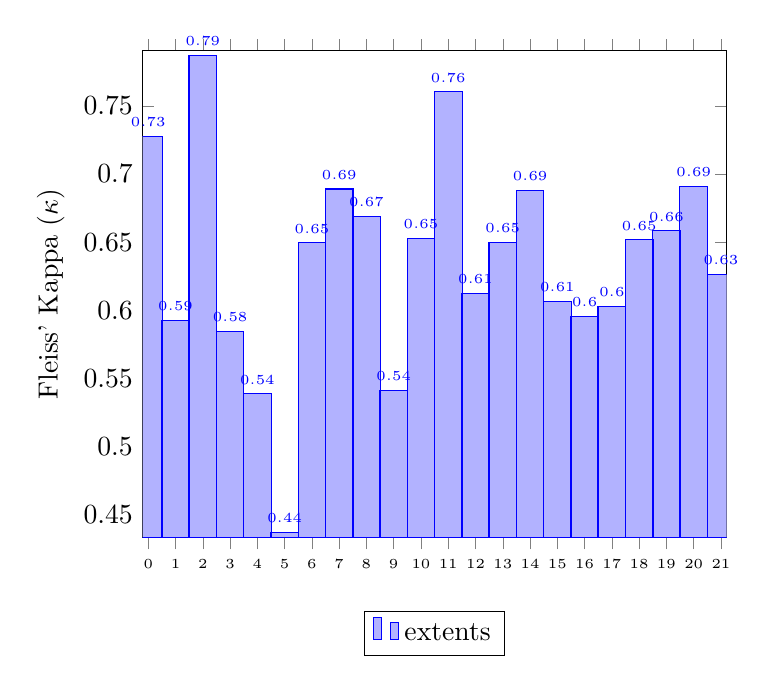
\begin{tikzpicture}
\begin{axis}[
    ybar,
    enlargelimits=0.01,
    legend style={at={(0.5,-0.15)},
      anchor=north,legend columns=-1},
    ylabel={Fleiss' Kappa ($\kappa$)},
    symbolic x coords={0,1,2,3,4,5,6,7,8,9,10,11,12,13,14,15,16,17,18,19,20,21},
    xtick=data, xticklabel style={font=\tiny},
    nodes near coords,
    every node near coord/.append style={font=\tiny},
    nodes near coords align={vertical},
    ]
\addplot coordinates {(0,0.727817235623) (1,0.592538358694) (2,0.78693376975) (3,0.584645806506) (4,0.538797814208) (5,0.436852461868) (6,0.649525469688) (7,0.689025281309) (8,0.668929736629) (9,0.54126153079) (10,0.652943662285) (11,0.760376697542) (12,0.612274466328) (13,0.650077459334) (14,0.687853221054) (15,0.606652052744) (16,0.595731324545) (17,0.60288782204) (18,0.651691287007) (19,0.658387934883) (20,0.691156421819) (21,0.626229085368) };
\legend{extents}
\end{axis}
\end{tikzpicture}
\end{frame}

\begin{frame}{Matched Extents}
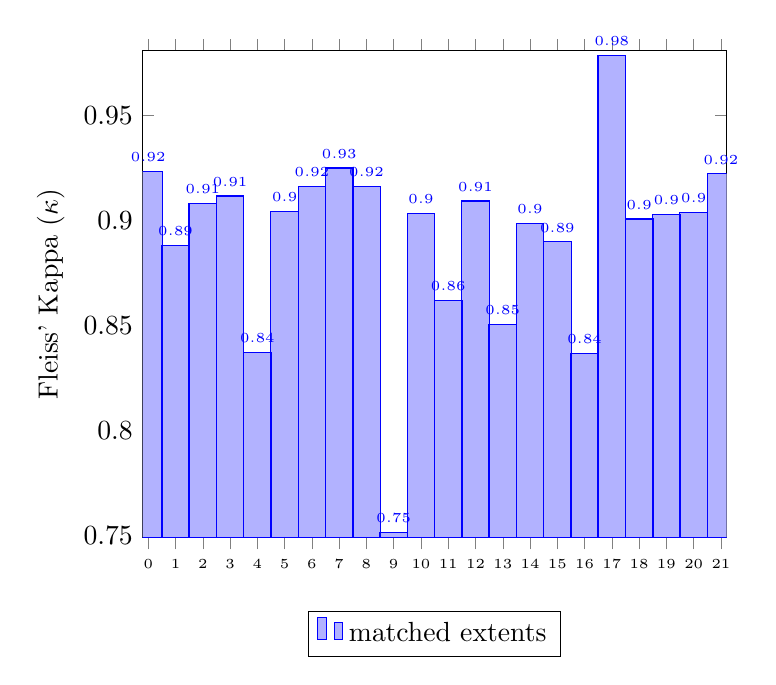
\begin{tikzpicture}
\begin{axis}[
    ybar,
    enlargelimits=0.01,
    legend style={at={(0.5,-0.15)},
      anchor=north,legend columns=-1},
    ylabel={Fleiss' Kappa ($\kappa$)},
    symbolic x coords={0,1,2,3,4,5,6,7,8,9,10,11,12,13,14,15,16,17,18,19,20,21},
    xtick=data, xticklabel style={font=\tiny},
    nodes near coords,
    every node near coord/.append style={font=\tiny},
    nodes near coords align={vertical},
    ]
\addplot coordinates {(0,0.923513766084) (1,0.88819167142) (2,0.908112351578) (3,0.911689335699) (4,0.837159871214) (5,0.904458598726) (6,0.916346564234) (7,0.925001847245) (8,0.916390264519) (9,0.751412429379) (10,0.903345724907) (11,0.861852433281) (12,0.909284725242) (13,0.850416171225) (14,0.898665795911) (15,0.889840905299) (16,0.836666666667) (17,0.97851453973) (18,0.900727763203) (19,0.902897112976) (20,0.903973152915) (21,0.922217720933) };
\legend{matched extents}
\end{axis}
\end{tikzpicture}
\end{frame}

\begin{frame}{Fleiss' Kappa for Tags}
\begin{adjustwidth}{-5em}{-3em}
\begin{figure}
\subfloat[hi]
{
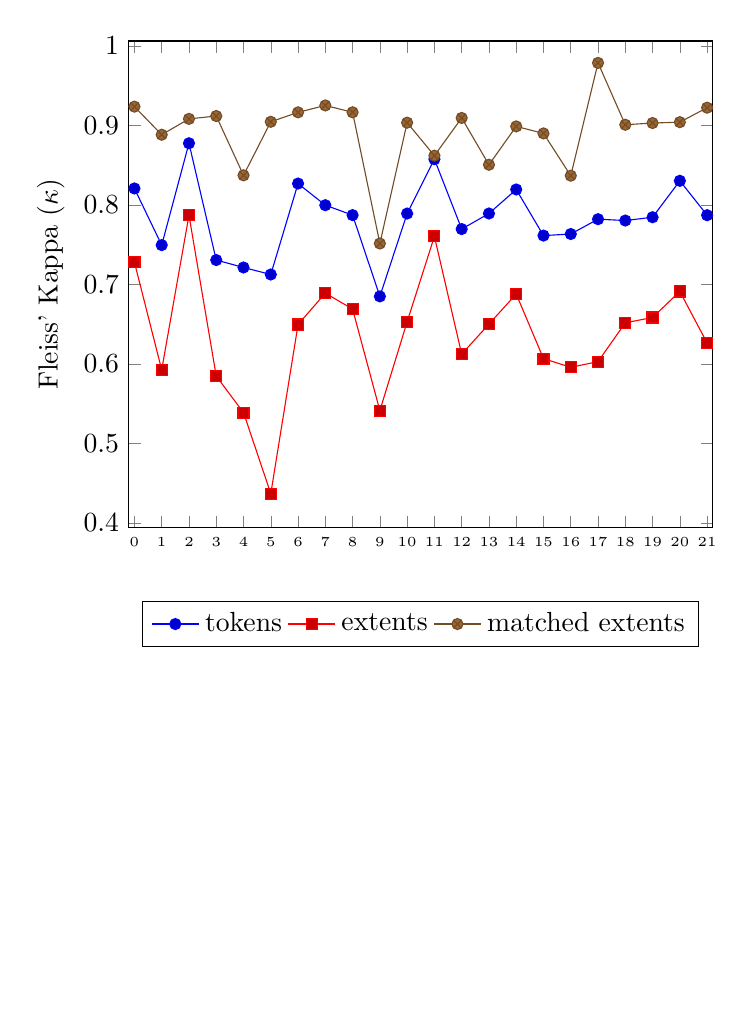
\begin{tikzpicture}[baseline = {(0,-5.75)}]
\begin{axis}[
    enlargelimits=0.01,
    legend style={at={(0.5,-0.15)},
      anchor=north,legend columns=-1},
    ylabel={Fleiss' Kappa ($\kappa$)},
    xtick=data,
    ymin = 0.4, ymax = 1, xticklabel style={font=\tiny}
    ]
\addplot coordinates {(0,0.820634615371) (1,0.749387104566) (2,0.877447627014) (3,0.730605521817) (4,0.721264576953) (5,0.712448104015) (6,0.826797749795) (7,0.799574244172) (8,0.787091644026) (9,0.684913627639) (10,0.789086760885) (11,0.857439617666) (12,0.769566208744) (13,0.789140742617) (14,0.819340189949) (15,0.761357917856) (16,0.763339845644) (17,0.781999988453) (18,0.780287210131) (19,0.784426418352) (20,0.830249577644) (21,0.786997332153) };
\addplot coordinates {(0,0.727817235623) (1,0.592538358694) (2,0.78693376975) (3,0.584645806506) (4,0.538797814208) (5,0.436852461868) (6,0.649525469688) (7,0.689025281309) (8,0.668929736629) (9,0.54126153079) (10,0.652943662285) (11,0.760376697542) (12,0.612274466328) (13,0.650077459334) (14,0.687853221054) (15,0.606652052744) (16,0.595731324545) (17,0.60288782204) (18,0.651691287007) (19,0.658387934883) (20,0.691156421819) (21,0.626229085368) };
\addplot coordinates {(0,0.923513766084) (1,0.88819167142) (2,0.908112351578) (3,0.911689335699) (4,0.837159871214) (5,0.904458598726) (6,0.916346564234) (7,0.925001847245) (8,0.916390264519) (9,0.751412429379) (10,0.903345724907) (11,0.861852433281) (12,0.909284725242) (13,0.850416171225) (14,0.898665795911) (15,0.889840905299) (16,0.836666666667) (17,0.97851453973) (18,0.900727763203) (19,0.902897112976) (20,0.903973152915) (21,0.922217720933) };
\legend{tokens,extents,matched extents}
\end{axis}
\end{tikzpicture}
}
\subfloat[yo]
{
\begin{tikzpicture}[baseline = {(0,-6)}]
    \node [draw,fill=white,anchor=north east] at (rel axis cs: 0.99,0.99) {\shortstack[l]{
        {\underline{Tasks Key}} \\
{\footnotesize 0 = 46\_N\_21\_E} \\{\footnotesize 1 = 48\_N\_27\_E} \\{\footnotesize 2 = 46\_N\_23\_E} \\{\footnotesize 3 = 48\_N\_12\_E} \\{\footnotesize 4 = 47\_N\_28\_E} \\{\footnotesize 5 = 48\_N\_10\_E} \\{\footnotesize 6 = 46\_N\_25\_E} \\{\footnotesize 7 = 46\_N\_22\_E} \\{\footnotesize 8 = 46\_N\_27\_E} \\{\footnotesize 9 = 47\_N\_26\_E} \\{\footnotesize 10 = 48\_N\_11\_E} \\{\footnotesize 11 = 46\_N\_24\_E} \\{\footnotesize 12 = 46\_N\_26\_E} \\{\footnotesize 13 = 47\_N\_27\_E} \\{\footnotesize 14 = 45\_N\_22\_E} \\{\footnotesize 15 = 47\_N\_25\_E} \\{\footnotesize 16 = 46\_N\_28\_E} \\{\footnotesize 17 = 47\_N\_24\_E} \\{\footnotesize 18 = 47\_N\_23\_E} \\{\footnotesize 19 = 45\_N\_23\_E} \\{\footnotesize 20 = 47\_N\_22\_E} \\{\footnotesize 21 = 48\_N\_8\_E}}}; 
\end{tikzpicture}
}
\end{figure}
\end{adjustwidth}
\end{frame}

\begin{frame}{Fleiss' Kappa for Tags (extents locked)}
\begin{adjustwidth}{-5em}{-3em}\begin{figure}\subfloat[hi]{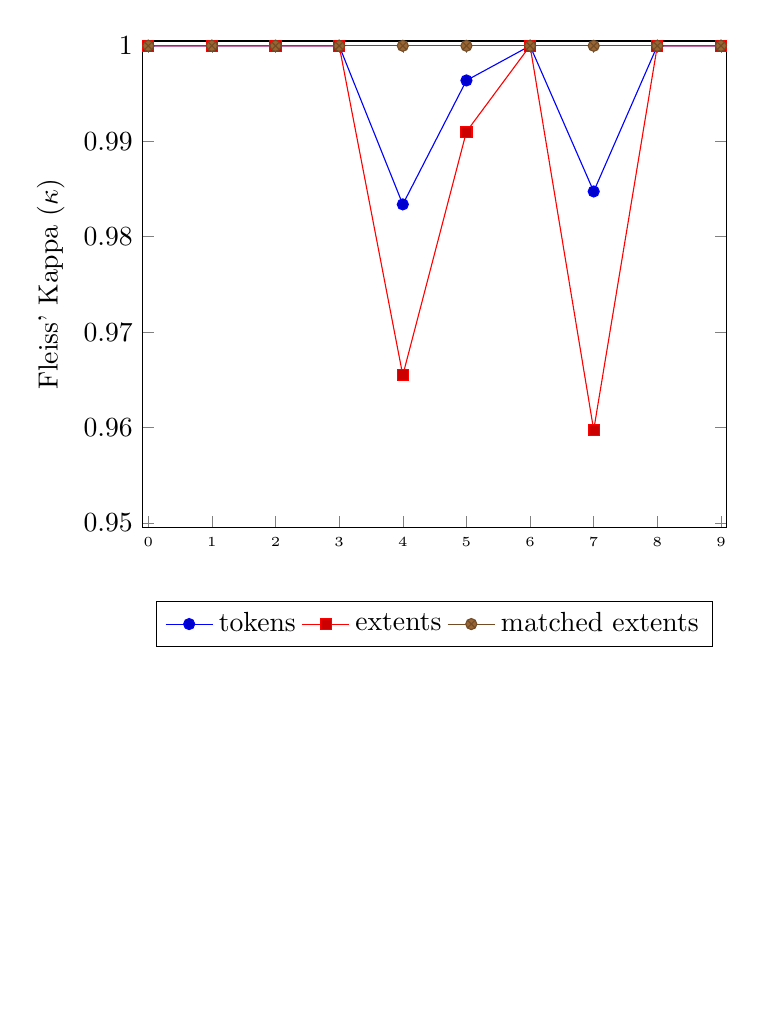
\begin{tikzpicture}[baseline = {(0,-5.75)}]
\begin{axis}[enlargelimits=0.01,legend style={at={(0.5,-0.15)},
            anchor=north,legend columns=-1}, ylabel={Fleiss' Kappa ($\kappa$)},
             xtick=data, ymin = 0.95, ymax = 1, xticklabel style={font=\tiny}]
\addplot coordinates {(0,1.0) (1,1.0) (2,1.0) (3,1.0) (4,0.983381824854) (5,0.996371080576) (6,1.0) (7,0.984737394193) (8,1.0) (9,1.0)  };
\addplot coordinates {(0,1.0) (1,1.0) (2,1.0) (3,1.0) (4,0.965479429801) (5,0.991000989891) (6,1.0) (7,0.959741120114) (8,1.0) (9,1.0)  };
\addplot coordinates {(0,1.0) (1,1.0) (2,1.0) (3,1.0) (4,1.0) (5,1.0) (6,1.0) (7,1.0) (8,1.0) (9,1.0)  };

\legend{tokens,extents,matched extents}\end{axis}
\end{tikzpicture}}\subfloat[yo]{\begin{tikzpicture}[baseline = {(0,-6)}]
                \node [draw,fill=white,anchor=north east] at (rel axis cs: 0.99,0.99) {\shortstack[l]{
             {\underline{\footnotesize{Tasks Key (extents locked)}}}\\{\footnotesize 0 = Transportation}\\{\footnotesize 1 = Medellin}\\{\footnotesize 2 = Bogota}\\{\footnotesize 3 = Floods}\\{\footnotesize 4 = IntoTheAndes}\\{\footnotesize 5 = Update}\\{\footnotesize 6 = Paramo}\\{\footnotesize 7 = Amazon}\\{\footnotesize 8 = PublicSchools}\\{\footnotesize 9 = PuertoOrdaz}}};\end{tikzpicture}}\end{figure}\end{adjustwidth}
\end{frame}

\begin{frame}{Document Length vs Fleiss' Kappa}
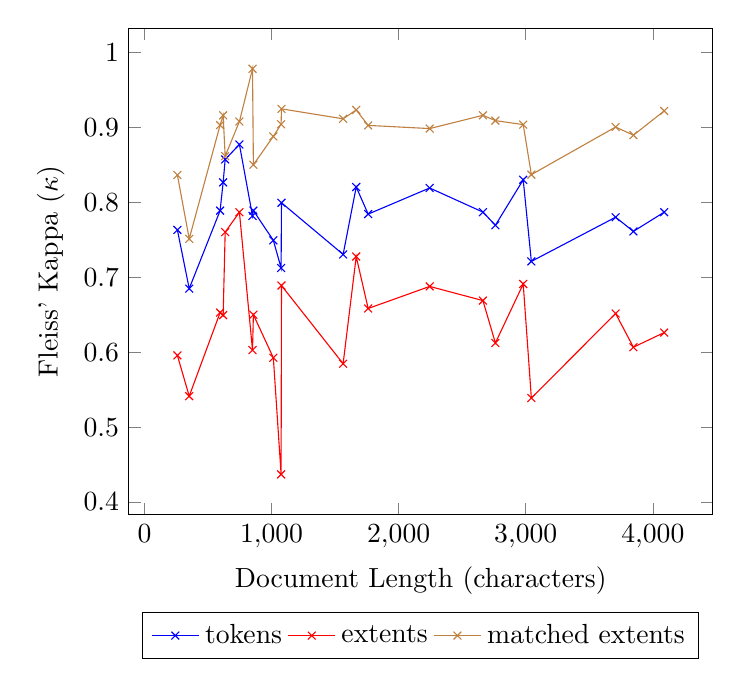
\begin{tikzpicture}
	\begin{axis}[
legend style={at={(0.5,-0.20)},
            anchor=north,legend columns=-1},
		xlabel=Document Length (characters),
		ylabel=Fleiss' Kappa ($\kappa$)]
\addplot[color=blue,mark=x] coordinates{(259,0.763339845644)(352,0.684913627639)(595,0.789086760885)(619,0.826797749795)(635,0.857439617666)(747,0.877447627014)(850,0.781999988453)(857,0.789140742617)(1014,0.749387104566)(1075,0.712448104015)(1078,0.799574244172)(1563,0.730605521817)(1666,0.820634615371)(1760,0.784426418352)(2244,0.819340189949)(2663,0.787091644026)(2761,0.769566208744)(2980,0.830249577644)(3044,0.721264576953)(3707,0.780287210131)(3847,0.761357917856)(4089,0.786997332153)};
\addplot[color=red,mark=x] coordinates{(259,0.595731324545)(352,0.54126153079)(595,0.652943662285)(619,0.649525469688)(635,0.760376697542)(747,0.78693376975)(850,0.60288782204)(857,0.650077459334)(1014,0.592538358694)(1075,0.436852461868)(1078,0.689025281309)(1563,0.584645806506)(1666,0.727817235623)(1760,0.658387934883)(2244,0.687853221054)(2663,0.668929736629)(2761,0.612274466328)(2980,0.691156421819)(3044,0.538797814208)(3707,0.651691287007)(3847,0.606652052744)(4089,0.626229085368)};
\addplot[color=brown,mark=x] coordinates{(259,0.836666666667)(352,0.751412429379)(595,0.903345724907)(619,0.916346564234)(635,0.861852433281)(747,0.908112351578)(850,0.97851453973)(857,0.850416171225)(1014,0.88819167142)(1075,0.904458598726)(1078,0.925001847245)(1563,0.911689335699)(1666,0.923513766084)(1760,0.902897112976)(2244,0.898665795911)(2663,0.916390264519)(2761,0.909284725242)(2980,0.903973152915)(3044,0.837159871214)(3707,0.900727763203)(3847,0.889840905299)(4089,0.922217720933)};
	\legend{tokens, extents, matched extents}
	\end{axis}
\end{tikzpicture}
\end{frame}

\begin{frame}{Fleiss' Kappa for QSLINK and OLINK}
\begin{adjustwidth}{-5em}{-3em}\begin{figure}\subfloat[hi]{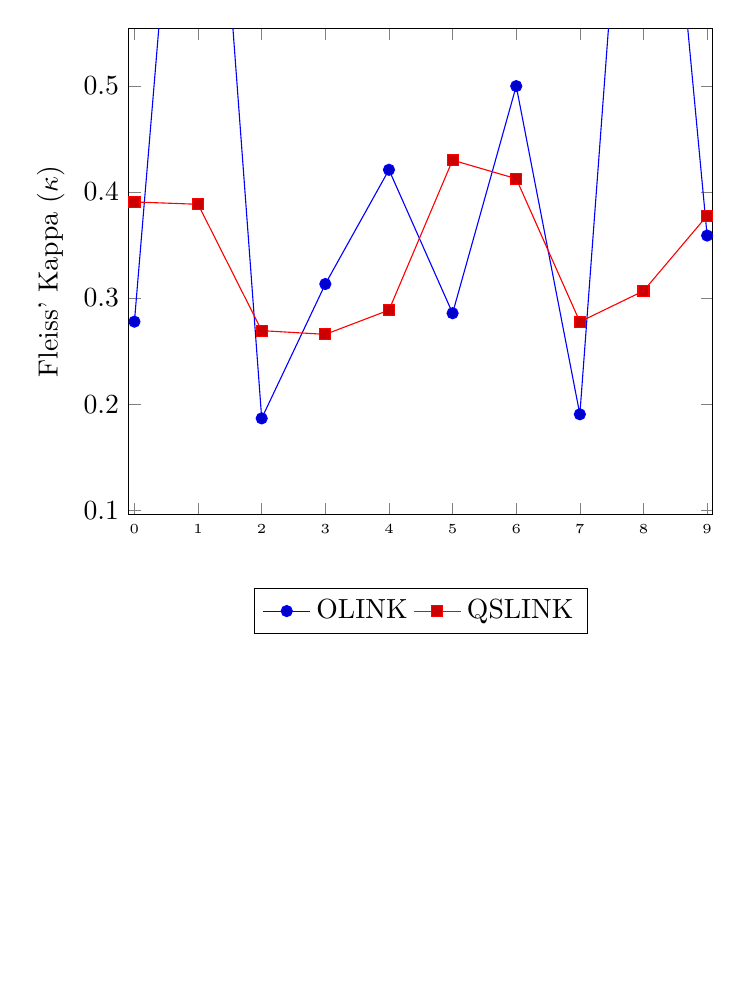
\begin{tikzpicture}[baseline = {(0,-5.75)}]
\begin{axis}[enlargelimits=0.01,legend style={at={(0.5,-0.15)},
            anchor=north,legend columns=-1}, ylabel={Fleiss' Kappa ($\kappa$)},
             xtick=data, ymin = 0.1, ymax = 0.55, xticklabel style={font=\tiny}]
\addplot coordinates {(0,0.277744715555) (1,1.0) (2,0.186540722342) (3,0.313260145109) (4,0.420991037641) (5,0.285709345508) (6,0.499917908304) (7,0.190377798889) (8,1.0) (9,0.358957691875)  };
\addplot coordinates {(0,0.390669781903) (1,0.388442170241) (2,0.269290857028) (3,0.265788703541) (4,0.288649924203) (5,0.430072614245) (6,0.412571848173) (7,0.277627283462) (8,0.306734351333) (9,0.377740442205)  };

\legend{OLINK,QSLINK}\end{axis}
\end{tikzpicture}}\subfloat[yo]{\begin{tikzpicture}[baseline = {(0,-6)}]
                \node [draw,fill=white,anchor=north east] at (rel axis cs: 0.99,0.99) {\shortstack[l]{
             {\underline{Tasks Key}}\\{\footnotesize 0 = Transportation}\\{\footnotesize 1 = Medellin}\\{\footnotesize 2 = Bogota}\\{\footnotesize 3 = Floods}\\{\footnotesize 4 = IntoTheAndes}\\{\footnotesize 5 = Update}\\{\footnotesize 6 = Paramo}\\{\footnotesize 7 = Amazon}\\{\footnotesize 8 = PublicSchools}\\{\footnotesize 9 = PuertoOrdaz}}};\end{tikzpicture}}\end{figure}\end{adjustwidth}
 \end{frame}

\end{document}